%--------------------
% Packages
% -------------------
\documentclass[11pt,a4paper]{article}


\usepackage[pdftex]{graphicx} % Required for including pictures
\usepackage[pdftex,linkcolor=black,pdfborder={0 0 0}]{hyperref} % Format links for pdf
\usepackage{calc} % To reset the counter in the document after title page

\frenchspacing % No double spacing between sentences
\linespread{1.2} % Set linespace
\usepackage[a4paper, lmargin=0.1666\paperwidth, rmargin=0.1666\paperwidth, tmargin=0.1111\paperheight, bmargin=0.1111\paperheight]{geometry} %margins

\usepackage[protrusion=true,expansion=true]{microtype} % Improves typography, load after fontpackage is selected


%-----------------------
% Set pdf information and add title, fill in the fields
%-----------------------
\hypersetup{
pdfsubject = {Software Product Engineering},
pdftitle = {SCEEM Space - OO Design and UML},
pdfauthor = {Jason Park, Sungijn Kang, William Nafack, Calum West}
}

%-----------------------
% Begin document
%-----------------------
\begin{document}

\begin{titlepage}
   \vspace*{\stretch{1.0}}
   \begin{center}
      \Large\textbf{SCEEM Space - OO Design and UML}\\
      \large\textit{Jason Park, Sungijn Kang, William Nafack, Calum West}
   \end{center}
   \vspace*{\stretch{2.0}}
\end{titlepage}

\section{OO Design and UML}
\subsection*{\bf Security}
After meeting with our client, we know that security is one of the main aspects of the system that will be most likely to affect our architecture. The web application itself must be secure as once you are logged on you will have access to information that is considered sensitive. Only certain members of staff are allowed to have access to this information, so our application needs to be structured as such that you cannot log-in without having a verified, authenticated login.
\bigskip

Our application itself will need a secure login system in which account details are encrypted and cannot be seen by anyone else. The way in which the sensitive information within the application itself is stored must also be secure as we do not want people to be able to access this through database consoles etc. 
\bigskip

Once students have graduated from the University their data needs to be deleted from the system so we need to make sure that this is done properly and in a way that it cannot be recovered. This will be done manually by members of staff. Data should also be kept up to date every single term to avoid issues with locating staff members or students. It is impossible to delete every bit of data by hand so we will need some functions that give the ability to delete all of the pieces of information associated with a particular person in the system.
\bigskip

We also want to be able to remove the verified logins of some staff members if they are to leave the University or are no longer given the permissions to be able to access the sensitive information.
\bigskip

\subsection*{\bf External systems}
For our product, we will be using H2 to store data and access data. We do not need to use a sign on feature 

When new students, staff, or academics enroll into the University, their data should be added into the database. Once they are added, there are different steps depending on whether they are staff or a student. For students and academics, some steps are required. First, they will be asked to designate their seats. Once this is done, staff members will check if their request is suitable or not (whether their request seat is close to their tutor, or their seat is in the same department section), then their seat will be decided. Another step is to give permission to book spaces. Only Kilim6519*
Kilim6519*
Kand academics can use this function. For members of staff, they can use most all the features of the web application. For example, they will be able to allocate seats to students and academics, whilst also being able to add and delete people from the system etc. Most of these things are all to do with the back-end of the system. This is the most important part of our project, so we should make sure all these functions work correctly, permissions of using them are given properly, and that data is secure. All these things are considered when making web application.
\bigskip

We also need to make a web page that shows all information to the user. There are four main sections that are going to be on the web app; Spaces, Persons, Waiting Lists, and Groups:

\begin{itemize}
    \item The ‘Spaces’ section will be the main section that will allow users to see information on all current spaces occupied by the school. The users will be able to find who is occupying different desks/offices, how many empty desks/offices there are, who is at a specific desk/office and so on.
    \item The ‘Persons’ section allows users to find all the information available about a specific person (academic, student, etc.). There will be a search function in which users can search for a person by some information about them, such as their name, research group or other.
    \item The ‘Waiting List’ section will show the waiting list for spaces and seats. When new people try to request their seat and spaces, they can see how many people are waiting for the same places. For new students and academics, they can request specific seats, and for all students, whenever they need spaces, they can request via this section.
    \item The ‘Groups’ section will show all the information available about any of the groups that the school sorts spaces for. Members of staff will be able to see how much space a specific group occupies and what buildings their students/academics are in.
\end{itemize}

This webpage will be the front-page. Users will not be able to directly access the database and directly edit the information stored in it. Since the website is where all the data will be managed by the users, it should be intuitive to use, and should be easy to navigate. If it is difficult to update/edit information, the project will be pointless as our main aim is to present the data that is currently difficult to interpret, in such a way that is easy on the eyes.
\bigskip

From a high-level architecture point of view, there are two main parts of our application; front end and back end. As previously mentioned, the front-end is the webpage that people will see and use, and the back-end is just the database and the interaction SpringBoot will have with the database. It is important that the front end and back end of our application work well together and are integrated well. For instance, when a person is removed from the system, all their data is removed and the seat they occupied will now be empty. Then this seat should be shown as empty on the webpage so that other people are able to see it as available and put in a request to be moved there. Users (students, academics, and staff) can only access and use the website. They cannot access the database directly. All the information updates will occur on the front-end, which will mean information has to be updated on the back end in the database. This updated information is then passed back to the front end to be displayed on the web page. The image below is a diagram outlining this high-level architecture:
\bigskip

It is highly likely that most users of the system will have no background in Computer Science. Therefore, we cannot ask them to just add data about staff/students straight into a database to then be manipulated by the web application. This example can also be applied to when they are logging in. Behind a simple looking login page, the logic can be very complicated. The username and password entered would be hashed with an encrypted version stored somewhere in a database containing all user logins. If this is successful then the user is granted access to the system. Usability of the service is the main reason we separate the front-end and the back-end from each other. 
\bigskip

\begin{figure}[!h]
    \centering
    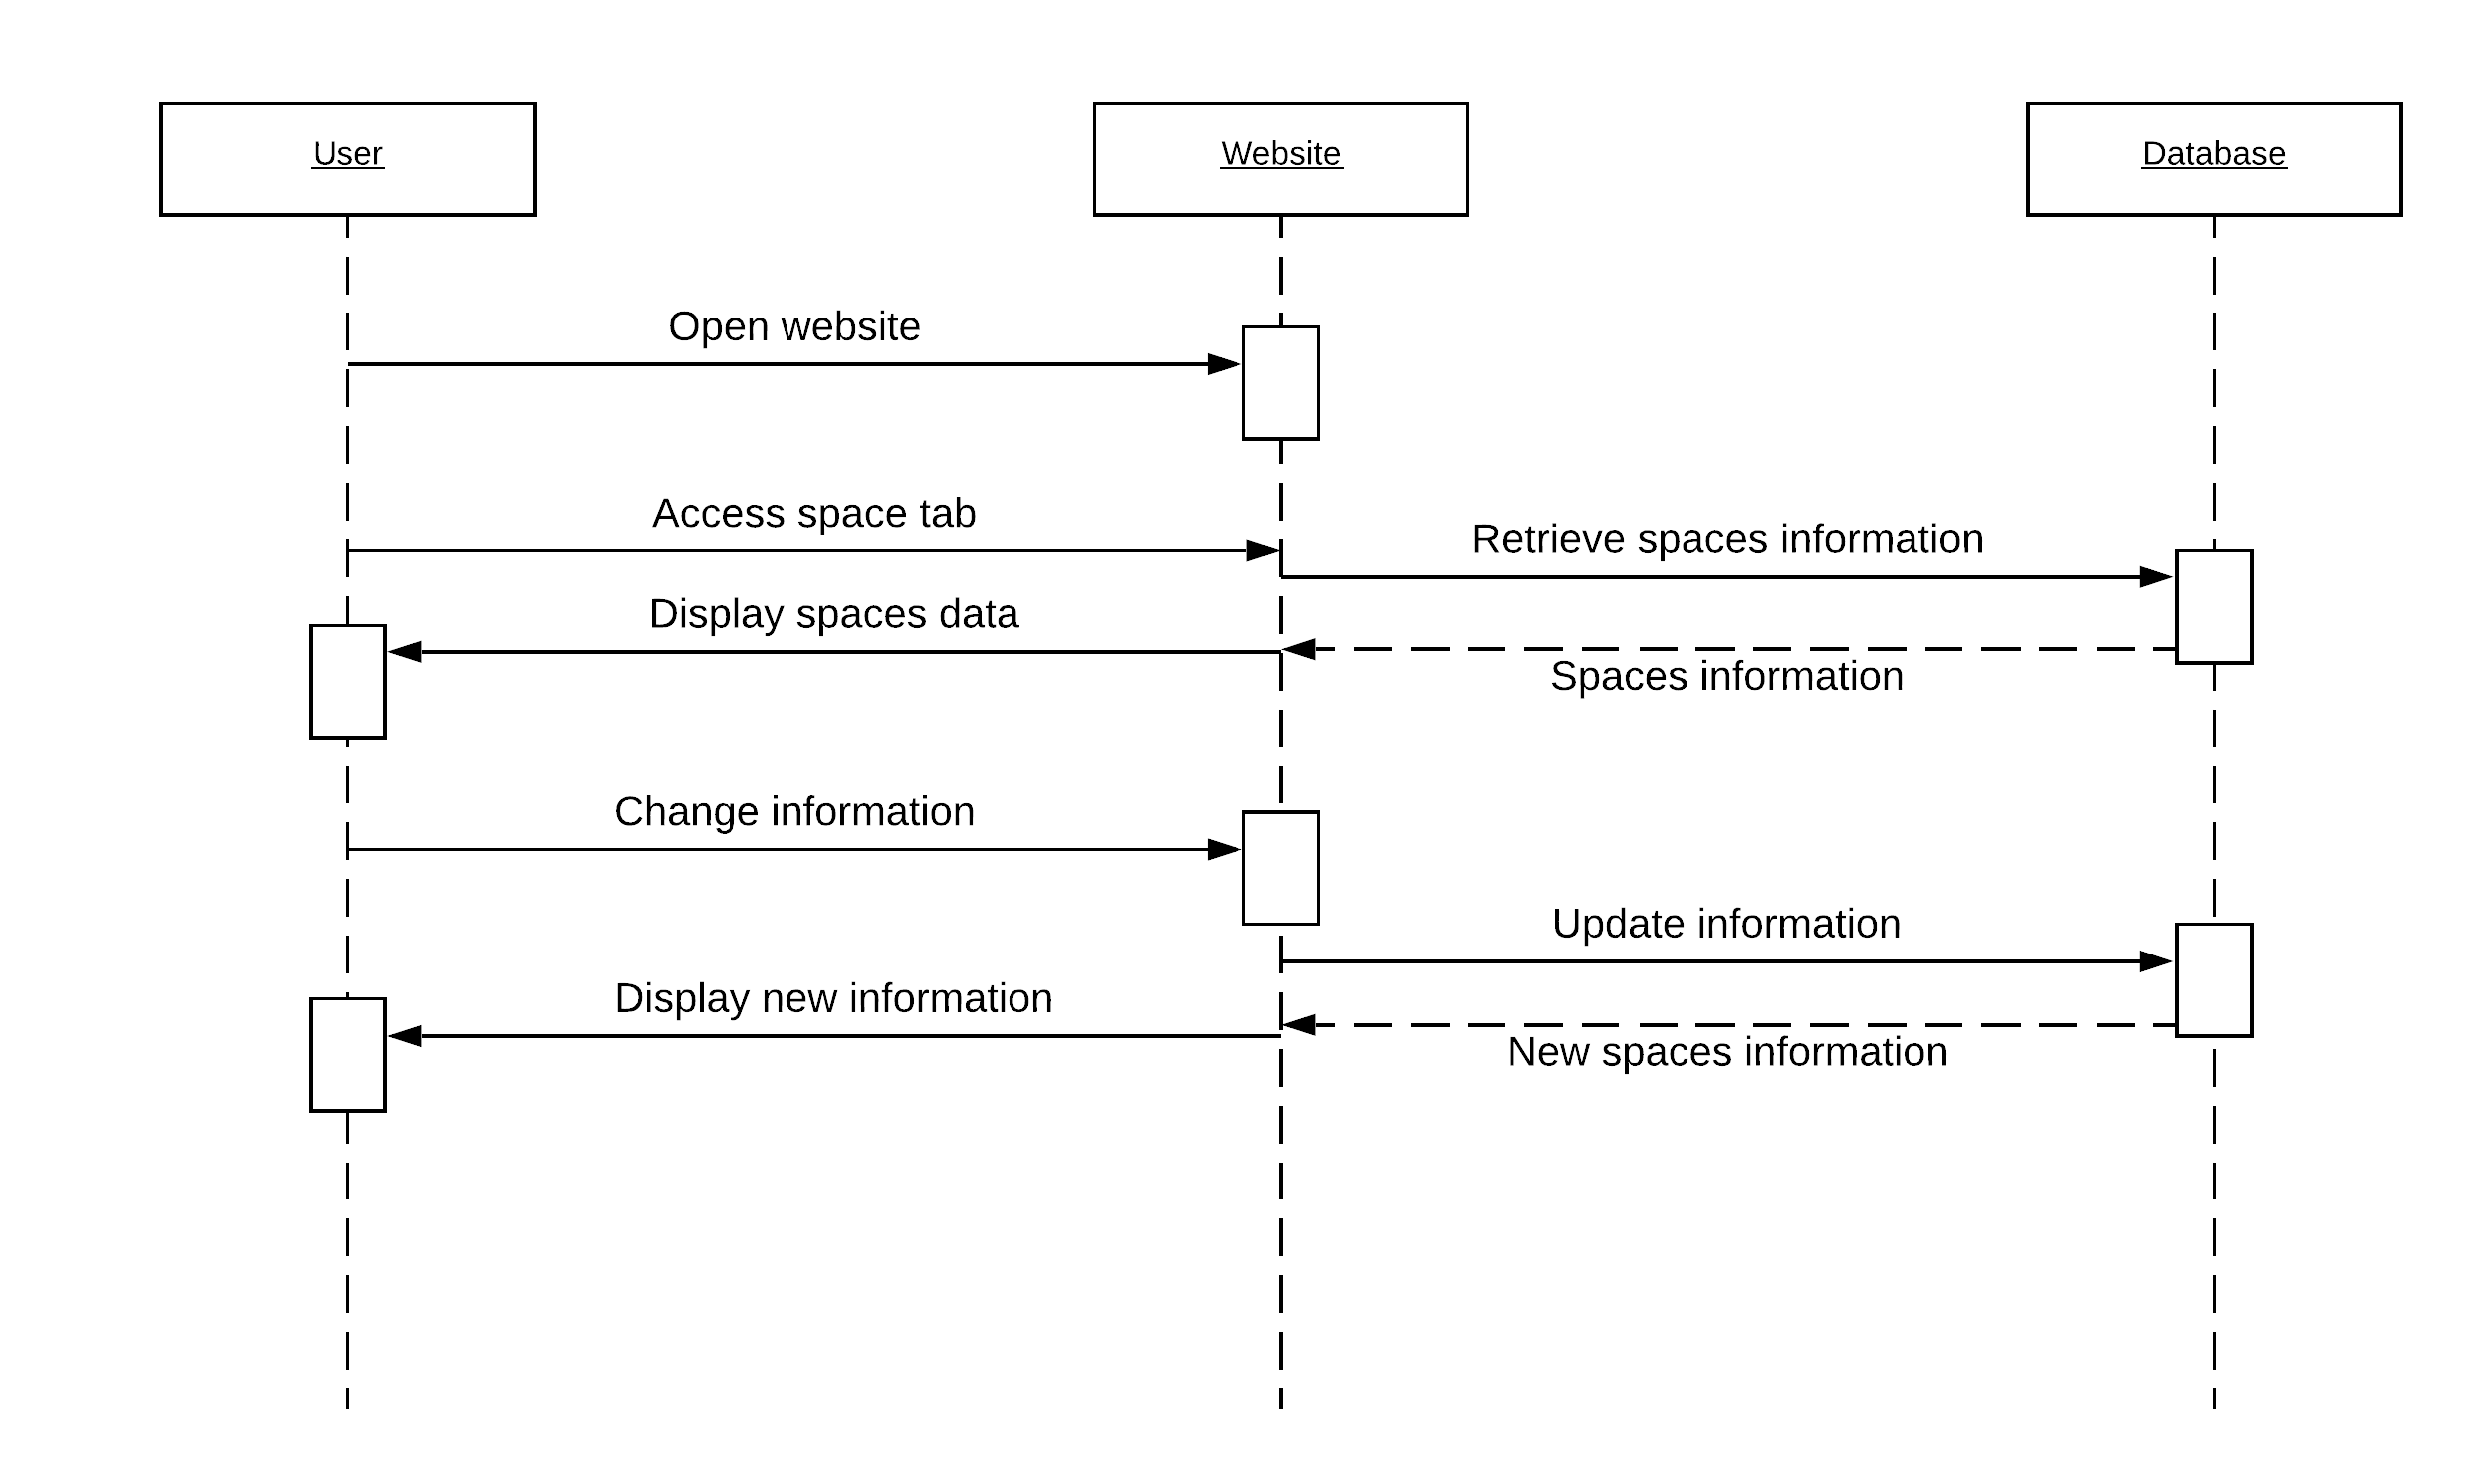
\includegraphics[width=\linewidth]{interaction.png}
    \caption{UML Interaction diagram}
    \label{fig:basic_2}
\end{figure}

This figure depicts a UML interaction diagram for a typical use case of our system. It depicts the use case where a user of the system opens the website and changes some information regarding an assigned space. This particular aspect is key to our system as this will be the most common use case so it is important that it is modelled in different types of diagram. Drawing out these designs in different kinds of diagrams also gives us a better understanding of how the system will work as a whole allowing us to better explain things to each other and the client.

\end{document}